%% This is free and unencumbered software released into the public domain.

%% Anyone is free to copy, modify, publish, use, compile, sell, or
%% distribute this software, either in source code form or as a compiled
%% binary, for any purpose, commercial or non-commercial, and by any
%% means.

%% In jurisdictions that recognize copyright laws, the author or authors
%% of this software dedicate any and all copyright interest in the
%% software to the public domain. We make this dedication for the benefit
%% of the public at large and to the detriment of our heirs and
%% successors. We intend this dedication to be an overt act of
%% relinquishment in perpetuity of all present and future rights to this
%% software under copyright law.

%% THE SOFTWARE IS PROVIDED "AS IS", WITHOUT WARRANTY OF ANY KIND,
%% EXPRESS OR IMPLIED, INCLUDING BUT NOT LIMITED TO THE WARRANTIES OF
%% MERCHANTABILITY, FITNESS FOR A PARTICULAR PURPOSE AND NONINFRINGEMENT.
%% IN NO EVENT SHALL THE AUTHORS BE LIABLE FOR ANY CLAIM, DAMAGES OR
%% OTHER LIABILITY, WHETHER IN AN ACTION OF CONTRACT, TORT OR OTHERWISE,
%% ARISING FROM, OUT OF OR IN CONNECTION WITH THE SOFTWARE OR THE USE OR
%% OTHER DEALINGS IN THE SOFTWARE.

%% For more information, please refer to <https://unlicense.org>
%%
\chapter{Functional Verification}\label{functionalverification}
Verification of electronic designs has become standard practice since the 1980
where the complexity of the design increased to the point that traditional test
methodologies could not scale as rapidly as the silicon progress. The general
estimation \cite{foster2015trends} shows that the functional verification
process takes more than 70\% of the overall project effort, representing the
primary bottleneck process in the hardware development. Verification can be seen
as an unbounded challenge in developing a product, where the only well-defined
goal is whether the circuit was subject to a set of inputs that exercised all
its functionality. This chapter describes and illustrates why functional
verification is needed and how it can be achieved.

\section{Why functional verification?}\label{sec:fv:why}
Verification as a process can be divided into several subcategories, from
manufacturing verification to formal verification, with each of them
accomplishing a specific goal. Perhaps the oldest one is the manufacturing
verification, in which a specific component is tested after it is produced. This
type of verification ensures that each device has an equivalent behavior as the
first device manufactured. Unlike manufacture verification, functional
verification attempts to verify that the hardware design operates as stated in
the specifications before the component is produced.

\par Nowadays, the cost to develop and manufacture a new hardware design is
considerably large, and ensuring its correctness before starting the production
is essential for limiting the fabrication costs. The trends reported in
\cite{mistry10nm}, shows the exponential jump in the number of transistors per
\SI{}{\milli\meter\squared} from one processor node to the next. Even though
nowadays, this jump in technology is happening less frequently than in the last
decade, the design potentials achievable from one generation to the next are
tremendously important. As an example, Intel's new \SI{10}{\nano\meter}
technology, only recently available to the consumer market, can take advantage
of up to \SI{100}{MTr/\milli\meter\squared} compared to the
\SI{37.5}{MTr/\milli\meter\squared} of the previous generation.

\begin{figure}[htb]
\centering
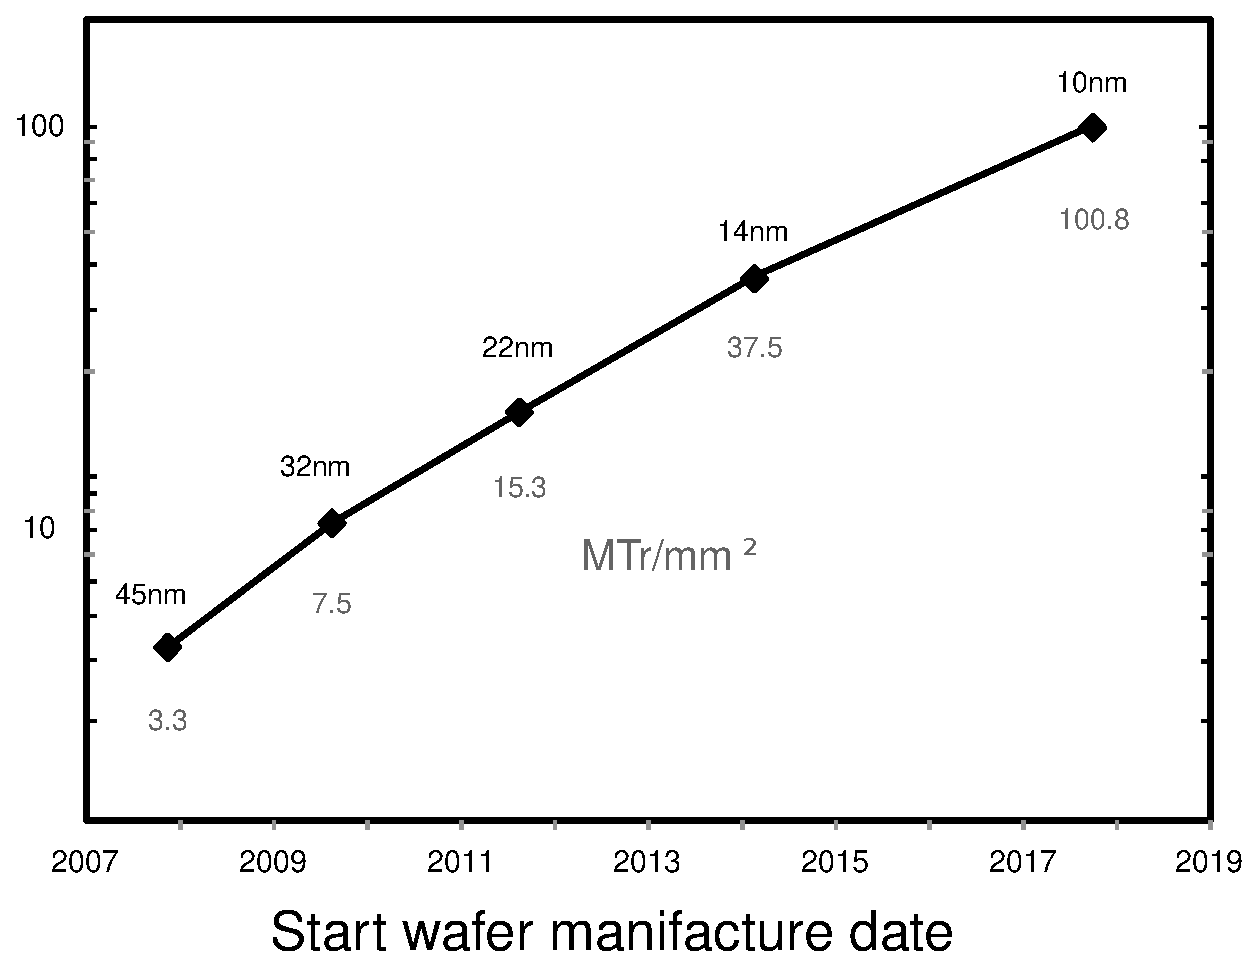
\includegraphics[width=0.7\linewidth]{pictures/Intel_scaling.eps}
\caption{Intel \si{MTr/mm^2} road-map \cite{mistry10nm}.}
\label{fig:ITMroadmap}
\end{figure}

\par Considering the picture \ref{fig:ITMroadmap}, it is necessary to remember
that the verification space grows exponentially compare to the design space. As
an example, a design consisting of 10 flip-flops, the number of internal states
needed to be verified in such design is 1024. By adding a single flip-flop, the
number of internal states doubles reaching 2048, and with it the verification
time needed to verify all the possible combinations of the flip-flops states.

\par While transistor's dimensions shrink and digital designers struggle to
maximize the new silicon technologies' design capability, the device complexity
increases, and with it the chances of mistakes and bugs. In the early days of
chip design, the verification of integrated an integrated circuit was done
manually by exercising the model and inspecting the waveforms to verify that it
behaved accordingly. This type of verification, known today as direct testing,
relies heavily on human inspection and thus is not scalable. By the end of the
1980s, the integrated circuit complexity made it impossible for the verification
engineers to exercise all aspects of a design in a reasonable amount of time,
and thus there was a need for a new methodology. After many iterations and
decades of trial, this shift in methodology led to what is known today as
functional verification.

\par In today's standards, it is common for a company to invest more time and
money in verification than in the actual design itself. Even with large
expenditures of money, integrated circuits are manufactured with several bugs,
and most of these imperfections are likely to be solved in software so as not to
compromise the release of the product. When the defects are unsolvable in
software, therefore requiring a redesign of the product, the hardware re-spin
cost is prone to surpass its revenue. A remarkable example is the Pentium FDIV
bug found in the Intel Pentium processor's floating-point unit in 1994
\cite{online:intelfvd}, which cost the company at the time around around US\$475
million, or US\$743 million today. The FDIV bug, other than being one of the
most remarkable examples, shows us that both the verification and product design
are human processes and are bound to have bugs.


\par To understand functional verification, it is vital to understand how the
design and the verification processes are related. The design process is the act
of converting the specifications into a detailed hardware description of the
product. By comparison, the verification process checks the designer's work by
addressing the same task from another perspective. While the design describes a
product's behavior from the inner to the outer, verification does the opposite,
verifying the behavior starting from the environment to the heart of the product
\cite{keating2011simple}. Ultimately, these two processes involve the human
factors, and both are prone to bugs. Figure
\ref{fig:whereverificationengineersspendtheirtime} shows us that verification
engineers spend as much time debugging their test benches as they spend writing
them. The ultimate goal in functional verification research is to eliminate as
much human factor as possible and improve the verification engineers'
efficiency.

\par Ideally, the number of verification engineers required per design engineer
is roughly estimated to be three to one. Unfortunately, this is rarely the case
in today's industry, and the statistics show that, most of the time, the number
are reversed \cite{foster2015trends}. For this reason, having a concrete
methodology and powerful verification tools that automate this process as much
as possible are essential to lower the gap between design and verification.

\begin{figure}[htb]
\centering
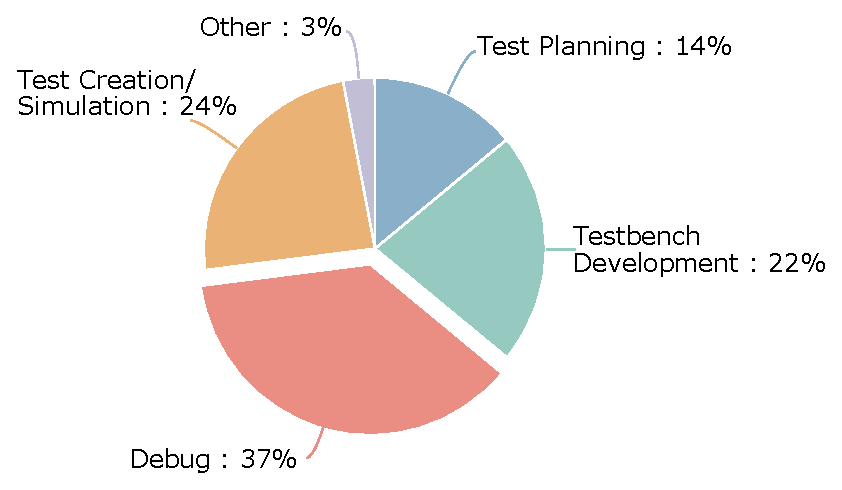
\includegraphics[width=0.8\linewidth]{pictures/Where_verification_engineers_spend_time.eps}
\caption{Where Verification Engineers Spend Their Time \cite{foster2015trends}.}
\label{fig:whereverificationengineersspendtheirtime}
\end{figure}

\section{What is functional verification?}
Fundamentally, functional verification can be seen as the process of comparing
two models describing the same component developed independently. If the two
models are developed separately from each other and their behavior matches in
all the aspects, it is safe to assume that both of them are correct. In digital
design, these two models are the model produced and developed by the design team
and the verification team, as described in section \ref{sec:fv:why}.

At the base of functional verification is a digital circuit expressed using
hardware description languages. A digital circuit can be defined as a
combinational circuit if its output is a pure and total function of its input.
On the other hand, a circuit is defined as sequential if its output depends on
the sequence of past inputs. Fundamentally, most of the digital circuits
developed today are sequential circuits. These type of circuits can be directly
reconducted into a finite state machine. A finite state machine, or FSM,
comprises several finite input, output, and internal states. By looking at the
amount of input, output, and internal control register present in the design, it
is possible to estimate its complexity or the size of its state space. A
state-space of a design can be defined as the set of all possible states of the
system \cite{definitionofstatespace}. As described by Lionel Bening and Harry D.
Foster in ``Principles of Verifiable RTL design" \cite{bening2001principles},
each RTL design can be represented as an FSM in which there are $m$ input
variables $x_0, x_1, \dots, x_{m-1}$, $n$-tuple output variables $z_0, z_1,
\dots, z_{n-1}$, the $p$-tuple of current state element variables $q_0, q_1,
\dots, q_{p-1}$, and the next-state variables $q_0^{'}, q_1^{'}, \dots,
q_{p-1}^{'}$.

\begin{figure}[htb]
\centering
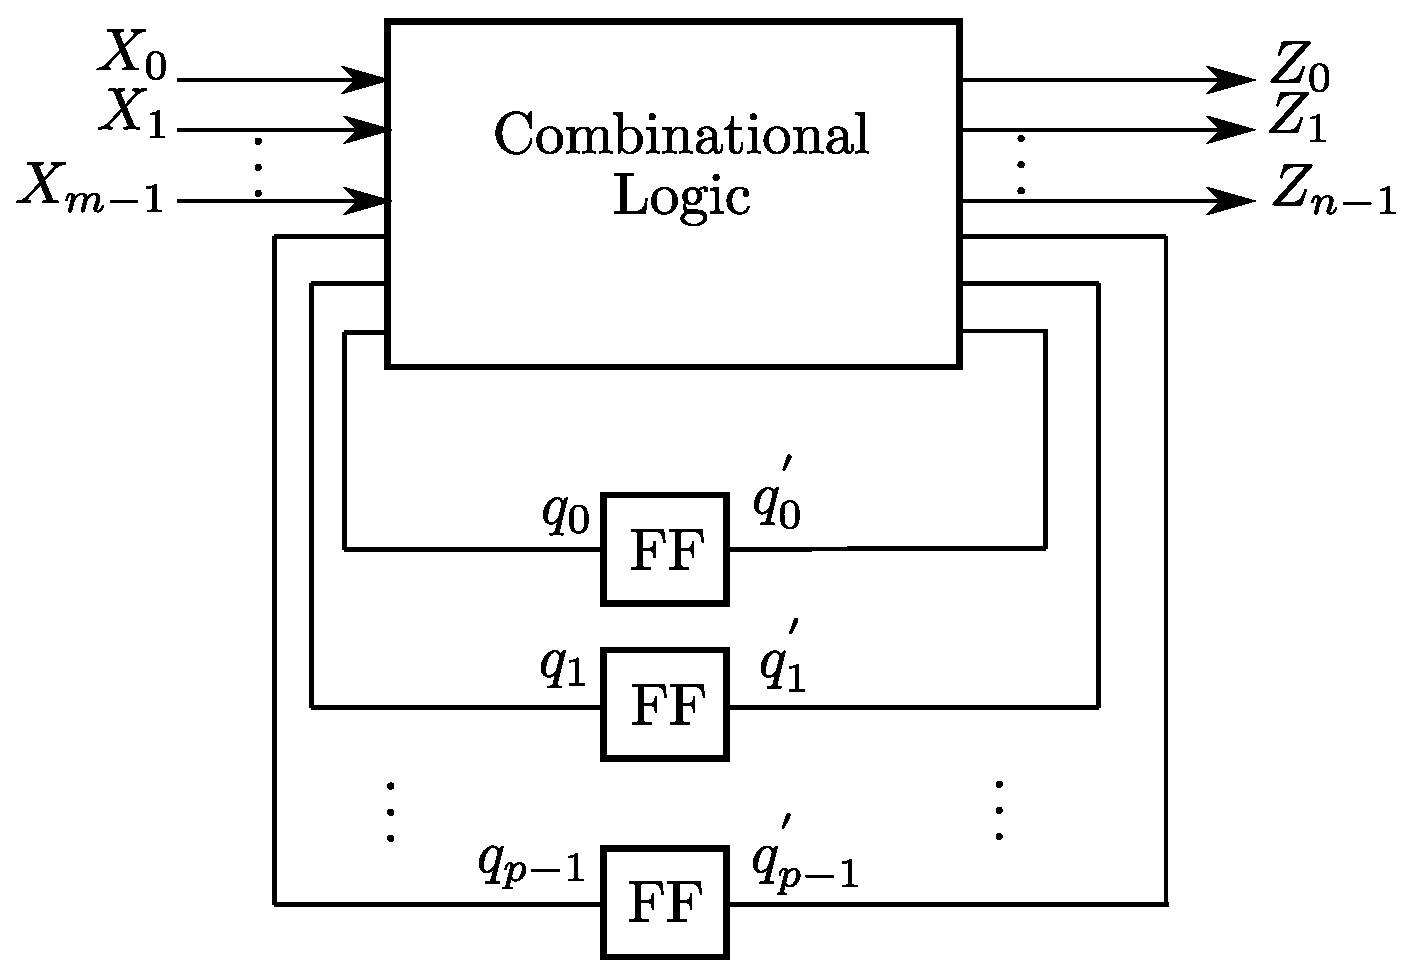
\includegraphics[width=0.6\linewidth]{pictures/Huffman_FSM.eps}
\caption{Huffman FSM Model \cite{bening2001principles}.}
\label{fig:huffmanfsm}
\end{figure}
Formally a state machine can be denoted as a 6-tuple
\begin{equation*}
    M = (X,Z,S,s_0,\delta,\lambda)
\end{equation*}

Where:

\begin{description}
    \item[$X$] : represent the machine's input state space, which is a set of
      $m$-tuple input vectors $\xi_i = x_0,x_1,\dots, x_{m-1} \in X$.
    \item[$Z$] : represents the machine's output space, which is a set of
      $n$-tuple output vectors $\eta_j = z_0, z_1,\dots,z_{n-1} \in Z$.
    \item[$S$] : represents the machine's reachable state space, which consists
      of the $p$-tuple set of state element variables $s_k =q_0,q_1,\dots,
      q_{p-1}$. The finite state machine has a maximum of $2^p$ possible states,
      however, not all states are necessarily reachable. Hence $S \subseteq s_0,
      s_1,\dots, s_{2^{p-1}}$.
    \item[$s_0$] : is the initial state.
    \item[$\delta$] : is a set of mapping functions from the present state of
      the machine to the next state based on the values of an input vectors
      $\xi_i \in X (0 \leq i \leq 2^m)$. In other words, $\delta : X \times S
      \to S$. For example, $q_j^{'} = \delta_j(\xi_i,s_k)$ where $(0 \leq p)$
      and $s_k \in S$ for $(0 \leq k \leq 2^{p-1})$.
    \item[$\lambda$] : is a set of mapping functions from the present state of
      the machine to an output variable $z_l(0\leq l \leq p)$ based on the
      values of an input vector $\xi\in X (0 \leq i \leq 2^m)$. In other words,
      $\lambda: X \times S \to Z$.
\end{description}

The FSM model of an RTL design is fundamentally the complete mathematical
representation of the circuit's behavior. Thus it allows verification engineers
and designers to use mathematical tools to reason about the model pragmatically.
Functionally to verify a digital design can be seen as the process of traversing
its state-space while checking that its behavior matches the specifications. In
principle, the amount of sate in a design $S_T$ can be calculated as:

\begin{equation}
    S_T = 2^m \cdot 2^n \cdot 2^p = 2^{m + n + p}.
\end{equation}

Where $m$, $n$, and $p$ are the number of input variables, output variables, and
the number of internal states, respectively.

\par At the beginning of the digital era, the verification engineer specifically
wrote a test, for each functionality and then manually verified that the model
behaved correctly for different input vectors. By current standards, the number
of input and output and the internal state of a design has become so large that
it is not possible to verify each of them manually. For these reasons, the
verification process is now expressed as the product of ``quality." What is the
quality to be achieved in the verification process? The verification quality is
globally expressed as the percentage of state space traversed during the
verification process.

While expressing the verification quality as the percentage of the state space
covered gives a more precise definition of ``done," it is also necessary to
record and understand which part of the state space has been explored. Tracking
which part of the state space was traversed is unavoidable because, given the
complexity of modern designs, different properties and features can be
orthogonal between each other, so the percentage value needs to be correlated
with the number of features tested. Thus, the verification engineers need to
visualize the entire functional state space and decide how much coverage needs
to be carried for each feature.

The desired coverage percentage can be reached using different techniques, but
all of them can be grouped into two main categories: techniques that uses
dynamic verification \ref{sec:ver:dynamic}, and techniques using static
verification \ref{sec:ver:static}.


\section{Dynamic Verification}\label{sec:ver:dynamic}
Dynamic verification is the process of proving a design's correctness by
simulating it and comparing its response against the specification. The
simulation process can be achieved with different tools, techniques, and
performances. Generally, the device's HDL description is transformed into an
intermediate language then compiled, executed, or interpreted along with a
verification environment. The verification environment provides an abstraction
of the conditions in which the device is supposed to operate; it also provides
the functions to stress the device with stimuli and records the response and the
coverage measurements \cite{piziali2007functional}.

\section{Static Verification}\label{sec:ver:static}
As devices' size increases, verification engineers are searching for faster
techniques to reduce the amount of stimuli vectors needed to verify a device.
Static verification, in contrast to dynamic verification, analyzes the behavior
of hardware through mathematical transformations. Given that a device's state
space can be expressed as a mathematical model, verification engineers can
formally verify designs' properties with the same medium. This mathematical
analysis is based on formally proving that a set of properties holds
unconditionally inside a device. Formal methods are powerful because they are
less reliant on the human factor in determining all the possible corner cases
that could trigger a specific bug \cite{piziali2007functional}. Using static
techniques in the verification process allows the verification engineer to find
bugs significantly earlier in the project development. Even though static
verification is as old as the dynamic one, only recently has it started to be
adopted by the industry. Static verification is a broad chapter in the
verification domain parallel to the dynamic one and is out of the thesis topic's
scope.

The next section introduces how the verification process was traditionally done
before the introduction of functional verification.

\section{Traditional Methodology}\label{sec:traditionalmethodology}
The term direct test or traditional methodology refers to how companies used to
verify integrated circuits before introducing functional verification. Direct
testing is the process of verifying a device by dynamically testing it and
comparing its behavior against a reference model. Before starting the
verification process, the verification engineers who use this methodology list
all the device features that need to be verified based on the design
specifications. After creating the list, the verification engineer defines how
many tests are necessary to thoroughly test each feature. This list of tests is
formally known as the verification plan. For each of the tests listed in the
verification plan, the verification engineer composes a vector of stimuli that
target a specific behavior to be verified. In the end, after simulating the
model, the log and waveforms produced are manually reviewed to ensure the design
behaved as expected \cite{spear2008systemverilog}.

\begin{figure}
\centering
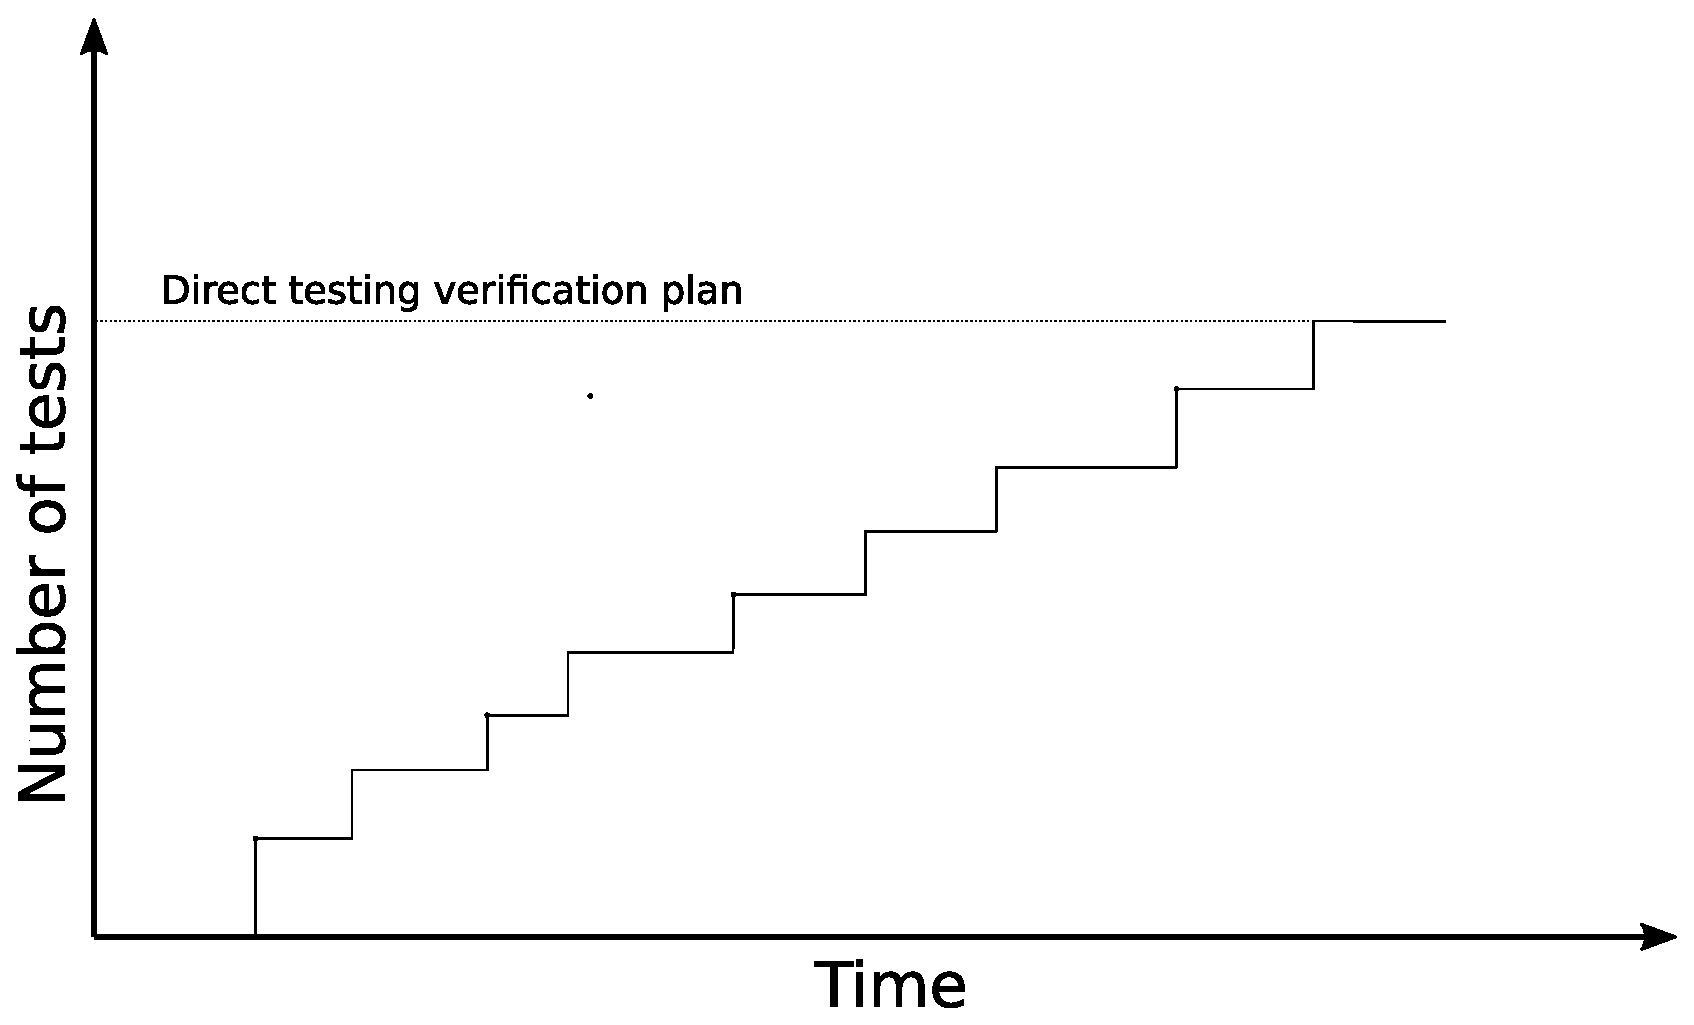
\includegraphics[width=0.6\linewidth]{pictures/Direct_testing.eps}
\caption{Direct testing progress over time \cite{spear2008systemverilog}.}
\label{fig:testingprogresstimedirect}
\end{figure}

Direct testing is an incremental approach in which every test needs to be
simulated and verified. Generally, verifying a device with only directed tests
is a human-intensive task, even for the most straightforward test. A more
pervasive problem with this approach is anticipating and modeling all the corner
cases and unexpected device behaviors. With direct testing, the verification
engineers can verify only the number of tests they can foresee. Given the high
level of parallelism achievable with hardware design, it is almost impossible to
predict all aspects of a particular model, leading to another problem: the
completeness criteria.

The completeness criteria are the ``done" criteria that determine when a device
is thoroughly tested. Commonly, with direct testing, the completeness criteria
are given by the verification plan. When all the tests listed in the test plan
are passed, the verification process is completed. Other than being difficult
for the verification engineers to detect all the possible corner case behaviors
of a device it is often problematic for them to keep up with the verification
plans since, in most cases, features are added continuously throughout the
design process. Thus the number of tests to be implemented rapidly grows, making
it hard to test all the possible combinations of input-output and internal
states of the model.

One important thing to note with direct testing is that each test in the
verification plan targets, implicitly, a specific or a group of states in the
model's state space. Because the information is implicit, the verification
engineers do not know which part and how much state space was covered. For this
reason, by using this empiric method, there is no way to ensure that the list of
tests in the verification plan crosses the entire state space of a model. Making
the matter worst is the fact that the waveform needs to be manually inspected
and verified, causing this process to be slow, human effort intensive, and
nondeterministic.

This methodology's limitations, combined with modern designs' complexity, lead
to the necessity of shifting the methodology towards a more deterministic
approach in which the coverage of the state space is expressed explicitly. This
new methodology is called Coverage Driven Verification and is the topic of the
next section.


\section{Coverage Driven Verification}\label{sec:covdrivenv}
As shown in the previous section, the traditional methodology of testing and
verifying a device does not scale with modern hardware design complexity. At the
end of the 20th century, the design space achievable by modern integrated
circuits made it impossible to traverse their entire state-space in a feasible
amount of time. These limitations, combined with the necessity of generating a
perfectly functional circuit at the first production cycle, made it necessary to
switch to a new methodology.

The new methodology requirements were precise from the beginning, and the final
goal was to find a method that scaled with the device complexity. As shown in
\cite{meyer2003principles}, the best verification quality equals to functionally
verify a device's correctness for the complete state space. When the total
state-space is too large to be inspected, the functional state-space can
directly translate to a new metric called Functional Coverage, which
encapsulates the state-space percentage currently verified in a design. With
this new metric, each direct test that, by nature, implicitly maps to a subset
of the state-space of model \ref{sec:traditionalmethodology} can now be
explicitly used to fulfill part of the functional coverage metric.

Functional Coverage is defined as the percentage of how many functionalities
were exercised during the verification process and is described with a Coverage
Model \cite{jain1995advanced}. A Coverage Model represents a family of shared
events that share common properties and thus are grouped into a model. Coverage
models are created by isolating similar properties of the design and collecting
them in groups called Cover Groups. Cover Groups are composed of smaller
elements called Coverage Bins. Each Cover Bin usually consists of a signal and a
set of values that this signal can take during the verification process.

Moreover, for each Cover Group, the verification engineer should define how to
sample each group. The sampling event can be defined as the rising edge of a
signal or a temporal expression, or a variable in the test bench. At the end of
the simulation, the verification engineer will look at the coverage report
emitted by the verification environment. The report usually contains the number
of times a valid value defined in the Cover Bin was encountered during the
verification process and the group's total Coverage percentage value.
Furthermore, it is then this total percentage that determines the new definition
of ``done."

Functional Coverage provides only information about which feature of the model
was executed while verifying the model. Thus, the correctness of the feature
needs to be verified against a reference model. It is also important to not
confuse Functional Coverage with Code coverage. While they both have a similar
purpose, Functional Coverage, as the name says, looks at how (in which order)
the model's functionalities were executed during the verification, where code
coverage tracks which part of the model was exercised.

Coverage metrics, like statement coverage and branch coverage, are quite large
topics and are not in the scope of this thesis. What is essential to understand
is that Functional Coverage gives the verification engineer a new metric
describing the completeness of the verification process for a specific design.

Even though moving from the traditional methodology to the new Functional
Coverage metrics gave a more precise definition of ``done," the verification
process was still highly bounded by the verification engineers' efficiency and
the number of tests written. Besides clarifying the definition of ``done,"
switching from an empirical verification model to a deterministic one exposes
the possibility of automatically generating random input vectors used to
stimulate the device. Random testing was not possible in the traditional
methodology because the verification engineer did not know which features were
tested using random inputs. By contrast, creating a testbench containing
functional probes like Cover Points and Cover Bins, allows to explicitly map
each test to a subset of the state space. Thus each random test is automatically
mapped to the overall Coverage Model contributing to the verification process's
coverage percentage.
 
This novel idea of randomizing the stimuli input vector is named Constrained
Random Verification or Coverage Driven Verification. The possibility of
automating stimulus is crucial for exercising intricate designs, where the
capabilities of the verification team cannot scale with the complexity of the
hardware. When automating stimuli are used in verification, there must be a
separation of concerns between the input vector's generation, the check of
correctness of a design, and the analysis of the completeness criteria. The
machine has to generate the tests without being aware of the correctness or
completeness criteria. With this methodology, the testbench itself is
responsible for verifying the generated tests' correctness while also sampling
the total Functional Coverage. Thus the generated tests should not carry
correctness and coverage information.
 
A remarkable property of randomly generated input vectors is its natural
predisposition to trigger the unknown aspect of a design not expected by
verification engineers. This property of random stimuli can be beneficial, but
it can also slow down the verification process by mostly hitting only portions
of the state space unreachable in the regular operation. For this reason, it is
necessary to constraint the randomness of the generated stimuli vector to only
the portion of state space that can be reachable during the regular operation of
a device. The next chapter introduces Random Constraint Verification and how it
is used in a modern verification environment.
